\chapter{評価}
\label{evaluation}
本章では,提案システムの評価に大きく二つ述べる。一つは他の活性化関数との比較。もう一つは、

\section{実験内容}
\subsubsection{実験1}

\subsubsection{実験3}
勾配が消失する条件について実験した。




\section{評価内容}



\subsection{既存の活性化関数との比較実験}



\subsubsection{実験1}

以下の条件で実験した。

\begin{table}[htbp]
    \begin{center}
        \caption{実験1の実行条件}
        \vspace{5mm} 
        \begin{tabular}{l*{2}{c}r}
        設定              & パラメータ \\
        \hline
        データセット            & ボストンの土地の価格 \\
        入力層 の次元            & 10 \\
        中間層 の次元            & 40 \\
        出力層 の次元            & 13 \\
        学習率              & 0.000001 \\
        勾配アルゴリズム       & SGD \\
        イニシャライザ               & kaiming normal \\
        ステップ数        & 200 \\
        ノーマライザー           & なし \\
        \end{tabular}
    \end{center}
\end{table}


\begin{figure}[hbtp]
    \begin{center}
        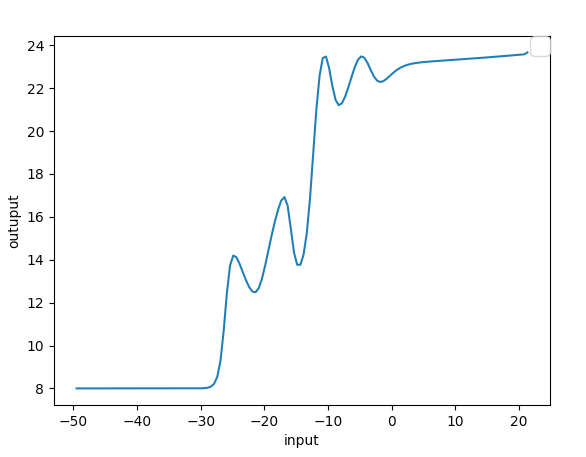
\includegraphics[width=10cm]{asset/boston_0000001_SGDkaiming_normal__non_200_function_2.png}
            \caption{活性化関数の形}
            \label{boston}
    \end{center}
\end{figure}


\begin{figure}[hbtp]
    \begin{center}
        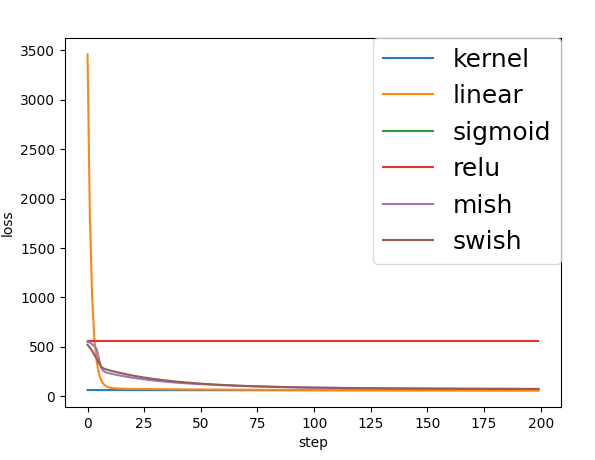
\includegraphics[width=10cm]{asset/boston_0000001_SGDkaiming_normal__non_200.png}
            \caption{Lossの比較データ}
            \label{boston}
    \end{center}
\end{figure}



\begin{table}[htbp]
    \begin{center}
        \caption{実験1の結果まとめ}
        \vspace{5mm} 
        \begin{tabular}{l*{2}{c}r}
            活性化関数              & loss \\
            \hline
            K-AF            & 0.0 \\
            Sigmoid            & -22.0 \\
            Linear            & 0.0 \\
            ReLU        & -22.0 \\
            Swish           & 0.0 \\
            Mish           & -1.0 \\
    
        \end{tabular}
    \end{center}
\end{table}




\section{まとめ}

K-AFの精度、勾配消失の有無、実用性の観点から先行研究との比較を行った. 実験結果を
踏まえ, 第 6 章で考察を行う.


%%% Local Variables:
%%% mode: japanese-latex
%%% TeX-master: "./thesis"
%%% End:
